\documentclass{beamer}
\usepackage{graphicx}
\usepackage{xcolor}
\usepackage{tikz}
\usepackage{amsmath}
\usepackage{pgfplots}
\pgfplotsset{compat=1.18}

\definecolor{purpleblue}{RGB}{80, 80, 180}
\definecolor{novelPurple}{RGB}{98, 54, 255}
\definecolor{softPurple}{RGB}{180, 170, 255}
\definecolor{softGray}{RGB}{235, 235, 245}
\definecolor{lightText}{RGB}{90, 90, 110}

\usetheme{Madrid}
\usecolortheme{dolphin}
\graphicspath{{static/course_materials/}{static/hard/}{./}}

\setbeamerfont{title}{size=\Large,series=\bfseries}
\setbeamerfont{frametitle}{size=\LARGE,series=\bfseries}
\setbeamercolor{frametitle}{fg=white, bg=novelPurple}
\setbeamercolor{title}{fg=white, bg=purpleblue}

\title[Test V]{\textbf{Test V}}
\author{\textbf{Jack Zeng}}
\institute{\textcolor{white}{\textbf{Novel Prep}}}
\date{\today}

\begin{document}

\begin{frame}
    \titlepage
    \vfill
    \begin{flushright}
        \textcolor{purpleblue}{\Huge \textbf{Novel Prep}}
    \end{flushright}
\end{frame}

\begin{frame}
    \begin{tikzpicture}[remember picture, overlay]
        \shade[top color=softPurple, bottom color=softGray]
            (current page.north west) rectangle (current page.south east);
        \node[align=center] at (current page.center) {
            {\Huge\bfseries\textcolor{purpleblue}{Novel Prep}} \\[0.5cm]
            {\Large\itshape\textcolor{lightText}{Phase 3 · Mock Exam Training}}
        };
    \end{tikzpicture}
\end{frame}

\begin{frame}{Overview}
    \tableofcontents
\end{frame}

\begin{frame}
\section{Test V}
    \begin{tikzpicture}[remember picture, overlay]
        \shade[top color=softPurple, bottom color=softGray]
            (current page.north west) rectangle (current page.south east);
        \node[align=center] at (current page.center) {
            {\LARGE\bfseries\textcolor{purpleblue}{Test V}} \\[0.5cm]
            {\Large\itshape\textcolor{lightText}{22 Module 2-style mock exam questions}}
        };
    \end{tikzpicture}
\end{frame}

% --- Question 1 ---
\begin{frame}{Question 1}
\small
\begin{center}
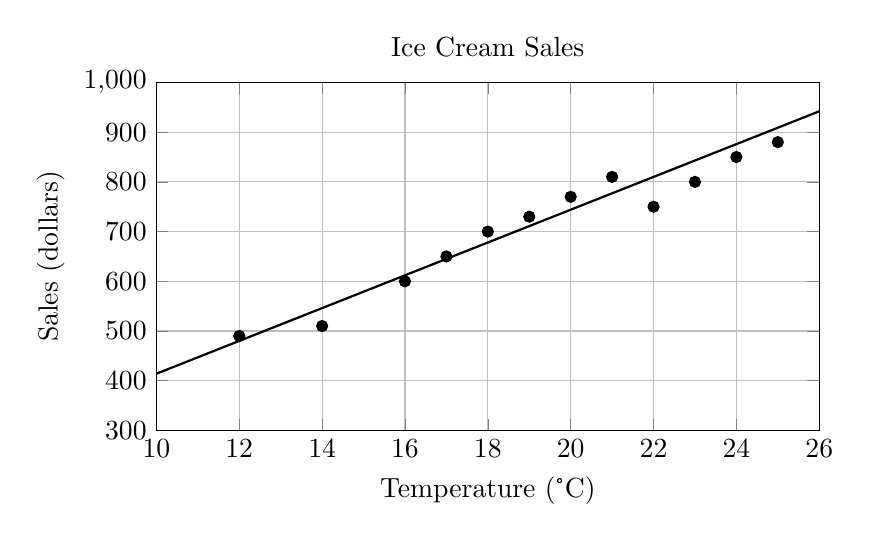
\begin{tikzpicture}
\begin{axis}[
    xlabel={Temperature (°C)},
    ylabel={Sales (dollars)},
    ytick={300,400,...,1000},
    xmin=10, xmax=26,
    ymin=300, ymax=1000,
    grid=major,
    width=10cm, height=6cm,
    title={Ice Cream Sales}
]
\addplot[
    only marks,
    mark=*,
]
coordinates {
    (12, 490)
    (14, 510)
    (16, 600)
    (17, 650)
    (18, 700)
    (19, 730)
    (20, 770)
    (21, 810)
    (22, 750)
    (23, 800)
    (24, 850)
    (25, 880)
};
\addplot[domain=10:26, thick] {33*x + 84};
\end{axis}
\end{tikzpicture}

\end{center}

The scatterplot above shows a company’s ice cream sales $d$, in dollars, and the high temperature $t$, in degrees Celsius (°C), on 12 different days.  
A line of best fit for the data is also shown.  
Which of the following could be an equation of the line of best fit?
\vspace{0.35cm}
\begin{enumerate}
    \item[A.] $d = 0.03t + 402$
    \item[B.] $d = 10t + 402$
    \item[C.] $d = 33t + 300$
    \item[D.] $d = 33t + 84$
\end{enumerate}
\end{frame}
\begin{frame}{Answer 1}
\small
\textbf{Correct Answer:} D
\end{frame}

% --- Question 2 ---
\begin{frame}{Question 2}
\small
The function \( F \) gives the temperature, in degrees Fahrenheit, that corresponds to a temperature of \( x \) kelvins. If a temperature increased by 10 kelvins, by how much did the temperature increase, in degrees Fahrenheit?

\[
F(x) = \frac{9}{5}(x - 273.15) + 32
\]
\end{frame}
\begin{frame}{Answer 2}
\small
\textbf{Final Answer:} $\boxed{18}$
\end{frame}

% --- Question 3 ---
\begin{frame}{Question 3}
\small
\begin{center}
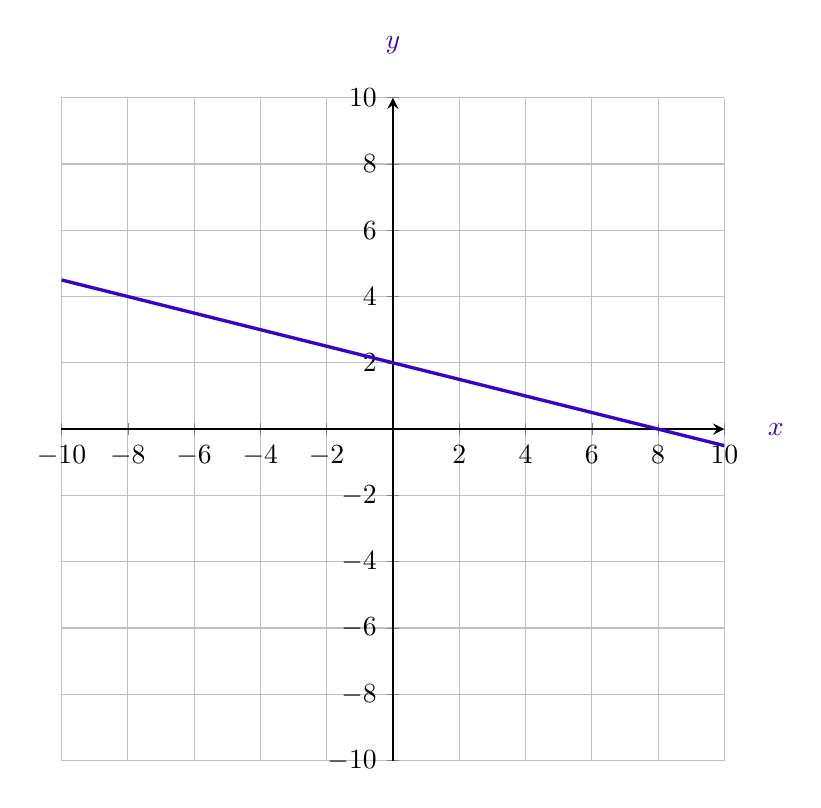
\begin{tikzpicture}
  \begin{axis}[
    axis lines=middle,
    % 紫蓝色刻度线
    xmin=-10, xmax=10,
    ymin=-10, ymax=10,
    xtick={-10,-8,...,10},
    ytick={-10,-8,...,10},
    grid=both,
    width=10cm,
    height=10cm,
    enlargelimits=false,
    xlabel={$x$}, ylabel={$y$},
    every axis x label/.style={
      at={(ticklabel* cs:1.05)}, anchor=west, color=purple!30!blue, font=\bfseries
    },
    every axis y label/.style={
      at={(ticklabel* cs:1.05)}, anchor=south, color=purple!30!blue, font=\bfseries
    },
    domain=-10:10,
    samples=2,
    thick
  ]
    \addplot [purple!30!blue, very thick] {-0.25*x + 2};
  \end{axis}
\end{tikzpicture}
\end{center}
The graph of \( y = f(x) + 14 \) is shown. Which equation defines function \( f \)?
\vspace{0.35cm}
\begin{enumerate}
    \item[A.] $f(x) = -\frac{1}{4}x - 12$
    \item[B.] $f(x) = -\frac{1}{4}x + 16$
    \item[C.] $f(x) = -\frac{1}{4}x + 2$
    \item[D.] $f(x) = -\frac{1}{4}x - 14$
\end{enumerate}
\end{frame}
\begin{frame}{Answer 3}
\small
\textbf{Correct Answer:} A
\end{frame}

% --- Question 4 ---
\begin{frame}{Question 4}
\small
A psychologist designed and conducted a study to determine whether playing a certain educational game  
increases middle school students’ accuracy in adding fractions.  
For the study, the psychologist chose a random sample of 35 students from all of the students  
at one of the middle schools in a large city. The psychologist found that students who played the game  
showed significant improvement in accuracy when adding fractions.  
What is the largest group to which the results of the study can be generalized?
\vspace{0.35cm}
\begin{enumerate}
    \item[A.] The 35 students in the sample
    \item[B.] All students at the school
    \item[C.] All middle school students in the city
    \item[D.] All students in the city
\end{enumerate}
\end{frame}
\begin{frame}{Answer 4}
\small
\textbf{Correct Answer:} B
\end{frame}

% --- Question 5 ---
\begin{frame}{Question 5}
\small
\begin{center}
\textbf{Poll Results}

\begin{tabular}{|l|c|}
\hline
Candidate & Votes \\
\hline
Jordan Lee & 552 \\
Maria Gomez & 451 \\
\hline
\end{tabular}
\end{center}

The table shows the results of a poll. A total of 1,003 voters selected at random were asked which candidate they would vote for in the upcoming election.  
According to the poll, if 8,240 people vote in the election, by how many votes would Jordan Lee be expected to win?
\vspace{0.35cm}
\begin{enumerate}
    \item[A.] 101
    \item[B.] 830
    \item[C.] 4,535
    \item[D.] 7,356
\end{enumerate}
\end{frame}
\begin{frame}{Answer 5}
\small
\textbf{Correct Answer:} B
\end{frame}

% --- Question 6 ---
\begin{frame}{Question 6}
\small
The function $f(x) = \frac{1}{9}(x - 7)^2 + 3$ gives a metal ball's height above the ground $f(x)$, in inches, $x$ seconds after it started moving, where $0 \leq x \leq 10$.  
What is the best interpretation of the vertex of the graph $y = f(x)$?
\vspace{0.35cm}
\begin{enumerate}
    \item[A.] The metal ball's minimum height was 3 inches above the ground.
    \item[B.] The metal ball's minimum height was 7 inches above the ground.
    \item[C.] The metal ball’s height was 3 inches above the ground when it started moving.
    \item[D.] The metal ball’s height was 7 inches above the ground when it started moving.
\end{enumerate}
\end{frame}
\begin{frame}{Answer 6}
\small
\textbf{Correct Answer:} A
\end{frame}

% --- Question 7 ---
\begin{frame}{Question 7}
\small
Given the system:  
\[
\begin{cases}
y = 2x^2 - 21x + 64 \\
y = 3x + a
\end{cases}
\]  
In the system of the equations, a is a constant. The graphs intersect at exactly one point \((x, y)\). What is the value of \(x\)?
\vspace{0.35cm}
\begin{enumerate}
    \item[A.] -8
    \item[B.] -6
    \item[C.] 6
    \item[D.] 8
\end{enumerate}
\end{frame}
\begin{frame}{Answer 7}
\small
\textbf{Correct Answer:} C
\end{frame}

% --- Question 8 ---
\begin{frame}{Question 8}
\small
Function $f$ is defined by $f(x) = (x + 6)(x + 5)(x + 1)$.  
Function $g$ is defined by $g(x) = f(x - 1)$.  
The graph of $y = g(x)$ in the $xy$-plane has $x$-intercepts at $(a, 0)$, $(b, 0)$, and $(c, 0)$, where $a$, $b$, and $c$ are distinct constants.  
What is the value of $a + b + c$?
\vspace{0.35cm}
\begin{enumerate}
    \item[A.] $-15$
    \item[B.] $-9$
    \item[C.] $11$
    \item[D.] $15$
\end{enumerate}
\end{frame}
\begin{frame}{Answer 8}
\small
\textbf{Correct Answer:} B
\end{frame}

% --- Question 9 ---
\begin{frame}{Question 9}
\small
For an online trivia game, 490 points are awarded for a correct answer if a question is answered in less than 5 seconds from the time the question is asked.  
Each 5 seconds after the question is asked, the number of points awarded for a correct answer decreases by 20\% of the number of points awarded for a correct answer in the previous 5 seconds.  

Which function gives the number of points awarded for a correct answer \(x\) seconds from the time the question is asked, where \(x\) is a multiple of 5?
\vspace{0.35cm}
\begin{enumerate}
    \item[A.] $f(x) = 490(0.80)^{\frac{x}{5}}$
    \item[B.] $f(x) = 490(0.80)^{5x}$
    \item[C.] $f(x) = 490(0.20)^{\frac{x}{5}}$
    \item[D.] $f(x) = 490(0.20)^{5x}$
\end{enumerate}
\end{frame}
\begin{frame}{Answer 9}
\small
\textbf{Correct Answer:} A
\end{frame}

% --- Question 10 ---
\begin{frame}{Question 10}
\small
A circle in the \(xy\)-plane has a diameter with endpoints \((a,11)\) and \((a,d)\), where \(a\) and \(d\) are constants.  

An equation of this circle is:  
\[
(x - a)^2 + (y - 17)^2 = r^2
\]  
where \(r\) is a positive constant.

What is the value of \(d\)?
\vspace{0.35cm}
\begin{enumerate}
    \item[A.] 5
    \item[B.] 12
    \item[C.] 17
    \item[D.] 23
\end{enumerate}
\end{frame}
\begin{frame}{Answer 10}
\small
\textbf{Correct Answer:} D
\end{frame}

% --- Question 11 ---
\begin{frame}{Question 11}
\small
One of the equations in a system of two linear equations is given:  
\[
31(x - n) = 31y + 31n
\]  
where \(n\) is a positive constant.  
The system has no solution. Which equation could be the second equation in this system?
\vspace{0.35cm}
\begin{enumerate}
    \item[A.] $3x - 3y = 6n$
    \item[B.] $3x + 3y = 3n$
    \item[C.] $3x + 3y = 6n$
    \item[D.] $3x - 3y = 3n$
\end{enumerate}
\end{frame}
\begin{frame}{Answer 11}
\small
\textbf{Correct Answer:} D
\end{frame}

% --- Question 12 ---
\begin{frame}{Question 12}
\small
In a mall, a person rides down an escalator, turns directly left at the base, and walks 16 feet (ft) to a kiosk.  
The escalator has a vertical rise of 18 ft and a horizontal run of 24 ft.  
If the person could have traveled in a straight line from the top of the escalator to the kiosk, what would the distance be, in feet?
\vspace{0.35cm}
\begin{enumerate}
    \item[A.] 24 ft
    \item[B.] 30 ft
    \item[C.] 34 ft
    \item[D.] 46 ft
\end{enumerate}
\end{frame}
\begin{frame}{Answer 12}
\small
\textbf{Correct Answer:} C
\end{frame}

% --- Question 13 ---
\begin{frame}{Question 13}
\small
The amount of money owed on a certain type of loan has two components: the principal balance of the loan and the amount of interest accrued on the loan.  
For a loan of this type, each payment was \$298.00 and there were 60 payments total. Part of each payment was applied to the principal balance of the loan, and the rest was applied to the amount of interest accrued on the loan.  
The amount of the 1st payment that was applied to the principal balance was \$220.93.  
For each additional payment, the amount that was applied to the principal balance was approximately 0.5\% greater than the amount that was applied to the principal balance for the previous payment.  

Which function best approximates the amount of the \(x\)th payment, in dollars, that was applied to the amount of interest accrued, where \(x \leq 60\)?
\vspace{0.35cm}
\begin{enumerate}
    \item[A.] $f(x) = 298.00 - 220.93(1.005)^{x-1}$
    \item[B.] $f(x) = 298.00 - 220.93(1.005)^{x}$
    \item[C.] $f(x) = (298.00 - 220.93)(0.995)^{x-1}$
    \item[D.] $f(x) = (298.00 - 220.93)(0.995)^x$
\end{enumerate}
\end{frame}
\begin{frame}{Answer 13}
\small
\textbf{Correct Answer:} A
\end{frame}

% --- Question 14 ---
\begin{frame}{Question 14}
\small
Right rectangular prism \(X\) is similar to right rectangular prism \(Y\).  
The surface area of right rectangular prism \(X\) is 52 square centimeters \((\text{cm}^2)\), and the surface area of right rectangular prism \(Y\) is 3,328 \(\text{cm}^2\).  
The volume of right rectangular prism \(X\) is 10.5 cubic centimeters \((\text{cm}^3)\).  

What is the volume, in \(\text{cm}^3\), of right rectangular prism \(Y\)?
\vspace{0.35cm}
\begin{enumerate}
    \item[A.] 1344
    \item[B.] 3328
    \item[C.] 5376
    \item[D.] 6656
\end{enumerate}
\end{frame}
\begin{frame}{Answer 14}
\small
\textbf{Correct Answer:} C
\end{frame}

% --- Question 15 ---
\begin{frame}{Question 15}
\small
A rectangular prism has a height of 50 centimeters (cm). The base of the prism is a square and the surface area of the prism is \( S \) cm\(^2\).  
If the prism is divided into two identical rectangular prisms by making a cut parallel to the square base, each resulting prism has a surface area of \(\frac{31}{50} S\) cm\(^2\).  

What is the side length, in cm, of each square base?
\end{frame}
\begin{frame}{Answer 15}
\small
\textbf{Final Answer:} $\boxed{\dfrac{600}{19}}$
\end{frame}

% --- Question 16 ---
\begin{frame}{Question 16}
\small
Two numbers, \( a \) and \( b \), are each greater than zero, and 4 times the square root of \( a \) is equal to 9 times the cube root of \( b \).  
If \( a = \left(\frac{2}{3}\right)^2 \), for what value of x that \( a^x \) is equal to \( b \)?
\end{frame}
\begin{frame}{Answer 16}
\small
\textbf{Final Answer:} $\boxed{\dfrac{9}{2}}$
\end{frame}

% --- Question 17 ---
\begin{frame}{Question 17}
\small
The expression \( kx \) represents the result of decreasing a positive force, \( x \), acting on an object by \( 0.34\% \). What is the value of \( k \)?
\vspace{0.35cm}
\begin{enumerate}
    \item[A.] \( 0.0034 \)
    \item[B.] \( 0.9966 \)
    \item[C.] \( 1.0034 \)
    \item[D.] \( 0.034 \)
\end{enumerate}
\end{frame}
\begin{frame}{Answer 17}
\small
\textbf{Correct Answer:} B
\end{frame}

% --- Question 18 ---
\begin{frame}{Question 18}
\small
A scientist studied the composition of one young swamp buffalo and determined the buffalo had 133 kilograms of muscle, which made up approximately 65.9\% of its composition. Of the remaining composition of this buffalo, approximately 46.2\% was bone, and the rest was fat.  

Based on these approximations, to the nearest tenth, how many kilograms of this buffalo’s composition was bone?
\end{frame}
\begin{frame}{Answer 18}
\small
\textbf{Final Answer:} $\boxed{31.8}$
\end{frame}

% --- Question 19 ---
\begin{frame}{Question 19}
\small
The function \( f \) is defined by \( f(x) = ax^2 + bx + c \), where \( a, b, \) and \( c \) are constants. The graph of \( y = f(x) \) in the \( xy \)-plane passes through the points \( (10, 0) \) and \( (-5, 0) \).  
If \( a \) is an integer greater than 1, which of the following could be the value of \( a + b \)?
\vspace{0.35cm}
\begin{enumerate}
    \item[A.] -8
    \item[B.] -4
    \item[C.] 5
    \item[D.] 6
\end{enumerate}
\end{frame}
\begin{frame}{Answer 19}
\small
\textbf{Correct Answer:} A
\end{frame}

% --- Question 20 ---
\begin{frame}{Question 20}
\small
In the equation \( y = bx(x - a)(x - a)(x + b)(x - b) \),  
\( a \) and \( b \) are positive constants and \( a \ne b \).  
How many distinct \( x \)-intercepts does the graph of the equation in the \( xy \)-plane have?
\vspace{0.35cm}
\begin{enumerate}
    \item[A.] Two
    \item[B.] Three
    \item[C.] Four
    \item[D.] Five
\end{enumerate}
\end{frame}
\begin{frame}{Answer 20}
\small
\textbf{Correct Answer:} C
\end{frame}

% --- Question 21 ---
\begin{frame}{Question 21}
\small
At different times on a certain day, a manager at a theme park recorded the number of visitors.  
An exponential model gives the estimated number of visitors, $V$, at the theme park $t$ hours after the theme park opened, where $t \leq 3$.  
Based on the model, 80 visitors were estimated to be at the theme park when it opened,  
and every 30 minutes the estimated number of visitors increased by 150\% of the number 30 minutes earlier.  
Which of the following equations best represents this model?
\vspace{0.35cm}
\begin{enumerate}
    \item[A.] $V = 80(2.5)^{2t}$
    \item[B.] $V = 80(2.5)^{\frac{t}{30}}$
    \item[C.] $V = 80(1.5)^{2t}$
    \item[D.] $V = 80(1.5)^{\frac{t}{30}}$
\end{enumerate}
\end{frame}
\begin{frame}{Answer 21}
\small
\textbf{Correct Answer:} A
\end{frame}

% --- Question 22 ---
\begin{frame}{Question 22}
\small
\begin{center}
    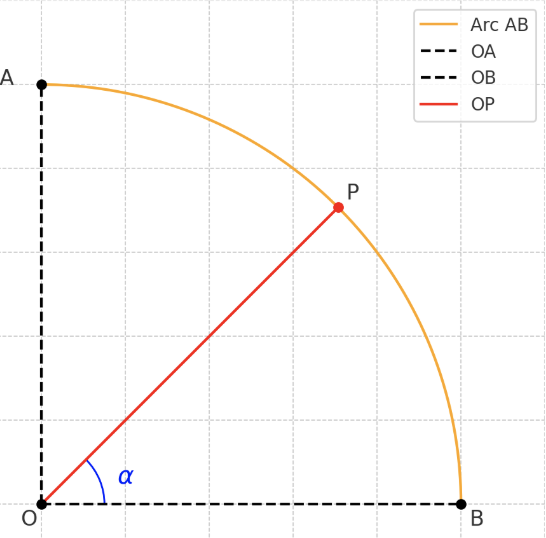
\includegraphics[width=0.5\linewidth]{hard_24_f11.png}
\end{center}
\textbf{As shown in the figure, \(O\) is the center of a circle with radius 1, and the circle intersects the coordinate axes at points \(A\) and \(B\).  
Point \(P\) lies on arc \(\overset{\frown}{AB}\) (not overlapping with \(A\) or \(B\)). Connect \(OP\), and let \(\angle POB = \alpha\).  
What are the coordinates of point \(P\)?}
\vspace{0.35cm}
\begin{enumerate}
    \item[A.] $(\sin\alpha, \sin\alpha)$
    \item[B.] $(\cos\alpha, \cos\alpha)$
    \item[C.] $(\cos\alpha, \sin\alpha)$
    \item[D.] $(\sin\alpha, \cos\alpha)$
\end{enumerate}
\end{frame}
\begin{frame}{Answer 22}
\small
\textbf{Correct Answer:} C
\vspace{0.15em}
\begin{columns}[T]
\begin{column}{0.38\textwidth}
\centering
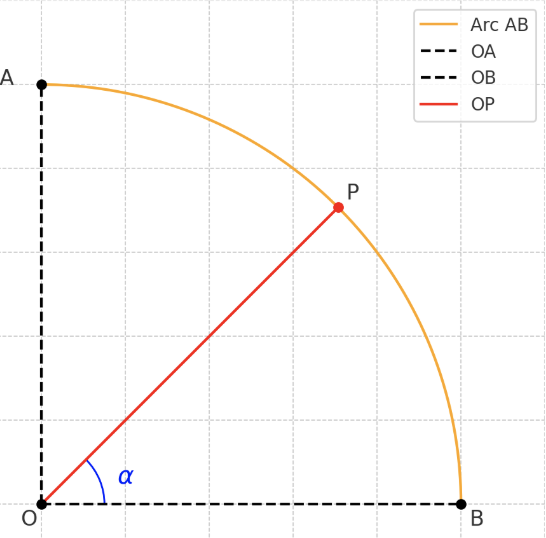
\includegraphics[width=\linewidth]{hard_24_f11.png}
\end{column}
\begin{column}{0.58\textwidth}
\footnotesize
Place $O$ at the origin with radius $1$: $A=(0,1)$, $B=(1,0)$.
$\angle POB=\alpha$ is measured from ray $\overrightarrow{OB}$
(the positive $x$-axis) to $\overrightarrow{OP}$.

On the unit circle,
\[
P=(\cos\alpha,\ \sin\alpha).
\]
Check: $\alpha=0\Rightarrow P=B=(1,0)$;
as $\alpha\to 90^\circ$, $P\to A=(0,1)$.

\textbf{Trap:} measuring from $\overrightarrow{OA}$ gives
$(\sin\alpha,\cos\alpha)$ (choice~D) --- wrong for this figure.
\end{column}
\end{columns}
\end{frame}

\begin{frame}{}
    \begin{tikzpicture}[remember picture, overlay]
        \shade[top color=novelPurple!40, bottom color=white]
            (current page.north west) rectangle (current page.south east);
        \fill[white, opacity=0.15] (current page.center) circle (5cm);
        \foreach \x in {1,2,3,4,5} {
            \fill[novelPurple, opacity=0.12] (rand*10-5, rand*7-3.5) circle (0.1+\x*0.05);
        }
    \end{tikzpicture}
    \centering
    \vspace{5em}
    {\Huge \textbf{\textcolor{novelPurple}{Thank You!}}} \\[1em]
    {\large \textcolor{gray}{We appreciate your time and focus.}} \\[3em]
    {\LARGE \textbf{\textcolor{novelPurple}{\textsf{Novel Prep}}}}
    \vfill
\end{frame}

\end{document}
